\subsection{Trip Planning: a natural-language planning extension}
\label{sec:results-trip}

The Countdown crossover should not be answered from arithmetic planning alone. Trip Planning therefore tests whether the same low-$k$/high-$k$ pattern persists under a stricter natural-language parser. The answer is yes in weaker but consistent form: Dream remains strongest among the standard diffusion runs at low $k$, while Llama benefits more from search and the flat-prompt Llama run becomes the strongest high-$k$ curve in the merged comparison. Deterministically, Dream variants occupy the top of the configuration ranking at $0.135$--$0.150$, with the next non-Dream model being LLaDA-Base at $0.115$ and the strongest AR model (Llama-Instruct flat) at $0.080$; the full ranked deterministic comparison across backends and block sizes is reproduced in Appendix~\ref{sec:appendix-trip-deterministic}.

\begin{figure}[!htbp]
\centering
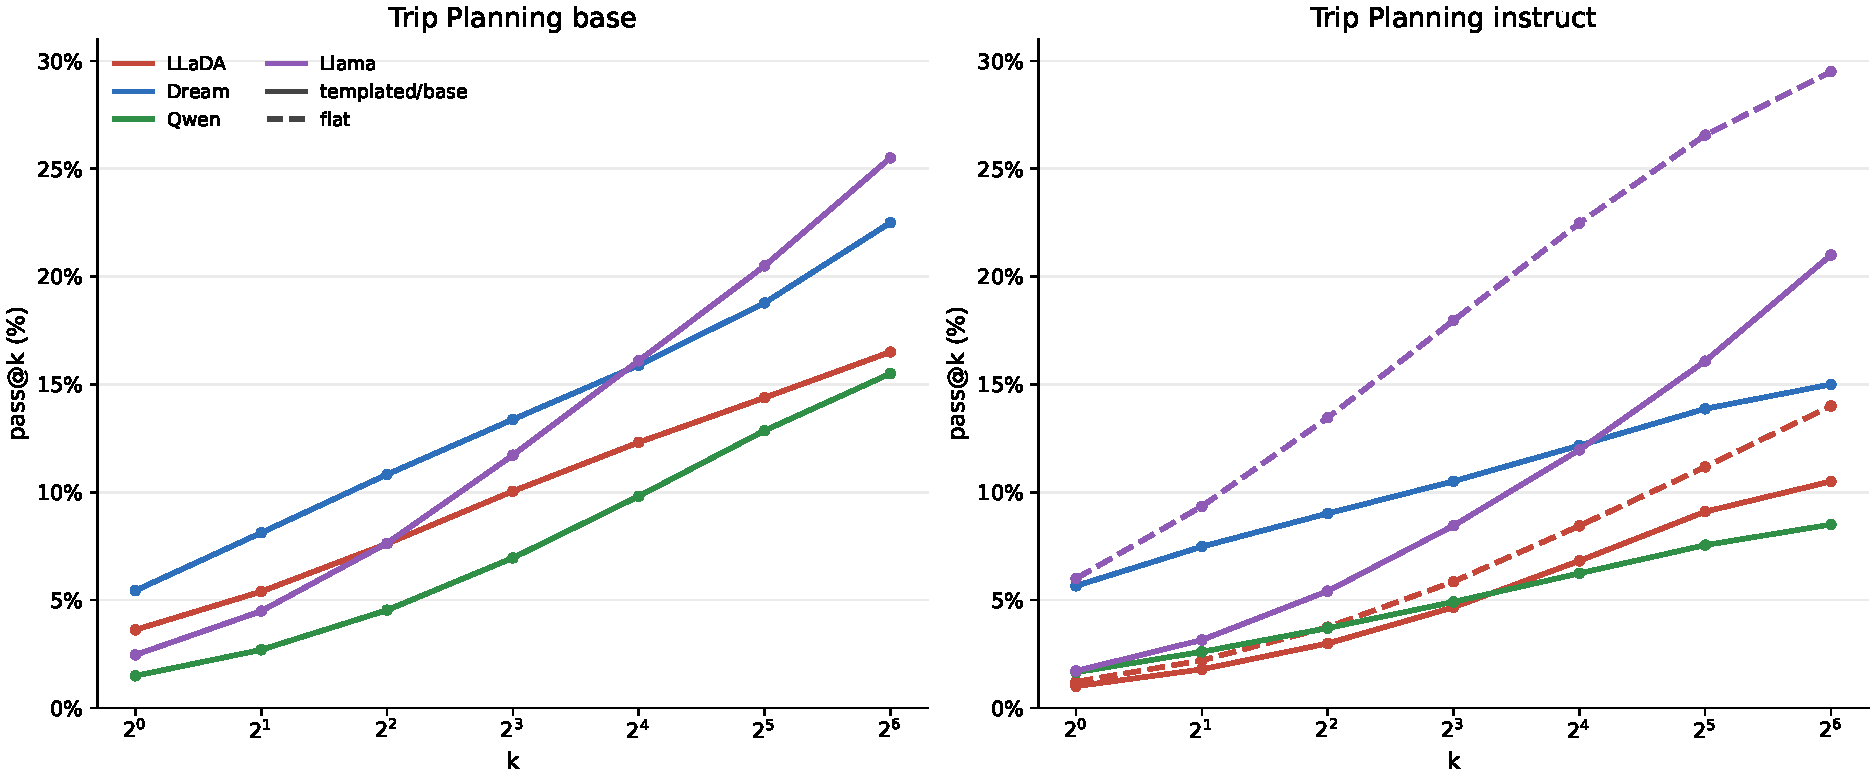
\includegraphics[width=0.94\textwidth]{images/trip_planning_passk.pdf}
\caption{Trip Planning pass@k for all stochastic milestone runs. Dream is strong at low $k$; Llama-Instruct flat has the strongest high-$k$ curve at pass@64$=0.295$.}
\label{fig:trip-passk}
\end{figure}

\begin{table}[!htbp]
\centering
\caption{Trip Planning pass@k, $n=64$, temperature $=0.7$, merged from Dream/Qwen, refreshed LLaDA, and Llama milestone sources.}
\label{tab:trip-passk}
\scriptsize
\resizebox{\textwidth}{!}{%
\begin{tabular}{lccccccc}
\toprule
\textbf{Model} & \textbf{1} & \textbf{2} & \textbf{4} & \textbf{8} & \textbf{16} & \textbf{32} & \textbf{64} \\
\midrule
Dream-Base & 0.054 & 0.081 & 0.108 & 0.134 & 0.159 & 0.188 & 0.225 \\
Dream-Instruct & 0.057 & 0.075 & 0.090 & 0.105 & 0.122 & 0.139 & 0.150 \\
LLaDA-Base & 0.036 & 0.054 & 0.076 & 0.100 & 0.123 & 0.144 & 0.165 \\
LLaDA-Instruct & 0.010 & 0.018 & 0.030 & 0.047 & 0.068 & 0.091 & 0.105 \\
LLaDA-Instruct flat & 0.012 & 0.022 & 0.037 & 0.059 & 0.084 & 0.112 & 0.140 \\
Qwen-Base & 0.015 & 0.027 & 0.045 & 0.070 & 0.098 & 0.129 & 0.155 \\
Qwen-Instruct & 0.016 & 0.026 & 0.037 & 0.049 & 0.062 & 0.075 & 0.085 \\
Llama-Base & 0.025 & 0.045 & 0.076 & 0.117 & 0.161 & 0.205 & 0.255 \\
Llama-Instruct & 0.017 & 0.031 & 0.054 & 0.084 & 0.120 & 0.161 & 0.210 \\
Llama-Instruct flat & 0.060 & 0.093 & 0.135 & 0.180 & 0.225 & 0.266 & 0.295 \\
\bottomrule
\end{tabular}}
\end{table}

Dream-Instruct and Dream-Base are the strongest standard diffusion curves at low $k$, while Llama-Instruct flat reaches $0.295$ at pass@64. The Trip Planning result is not identical to Countdown because the flat prompt changes Llama substantially, but the lesson is the same: single-sample and many-sample evaluations answer different questions, and the strongest model under one protocol is not the strongest under the other.
